\section{Feature matrix} 
Finally, the evaluation results of three platforms are put together and incorporated into the feature matrix as an Excel table. The complete feature matrix can be found in the appendix. Figure \ref{fig:featurematrix} shows the general structure of the matrix.
\newpage

\begin{figure}[h]
	\begin{adjustwidth}{-1.5cm}{}
	\centering
	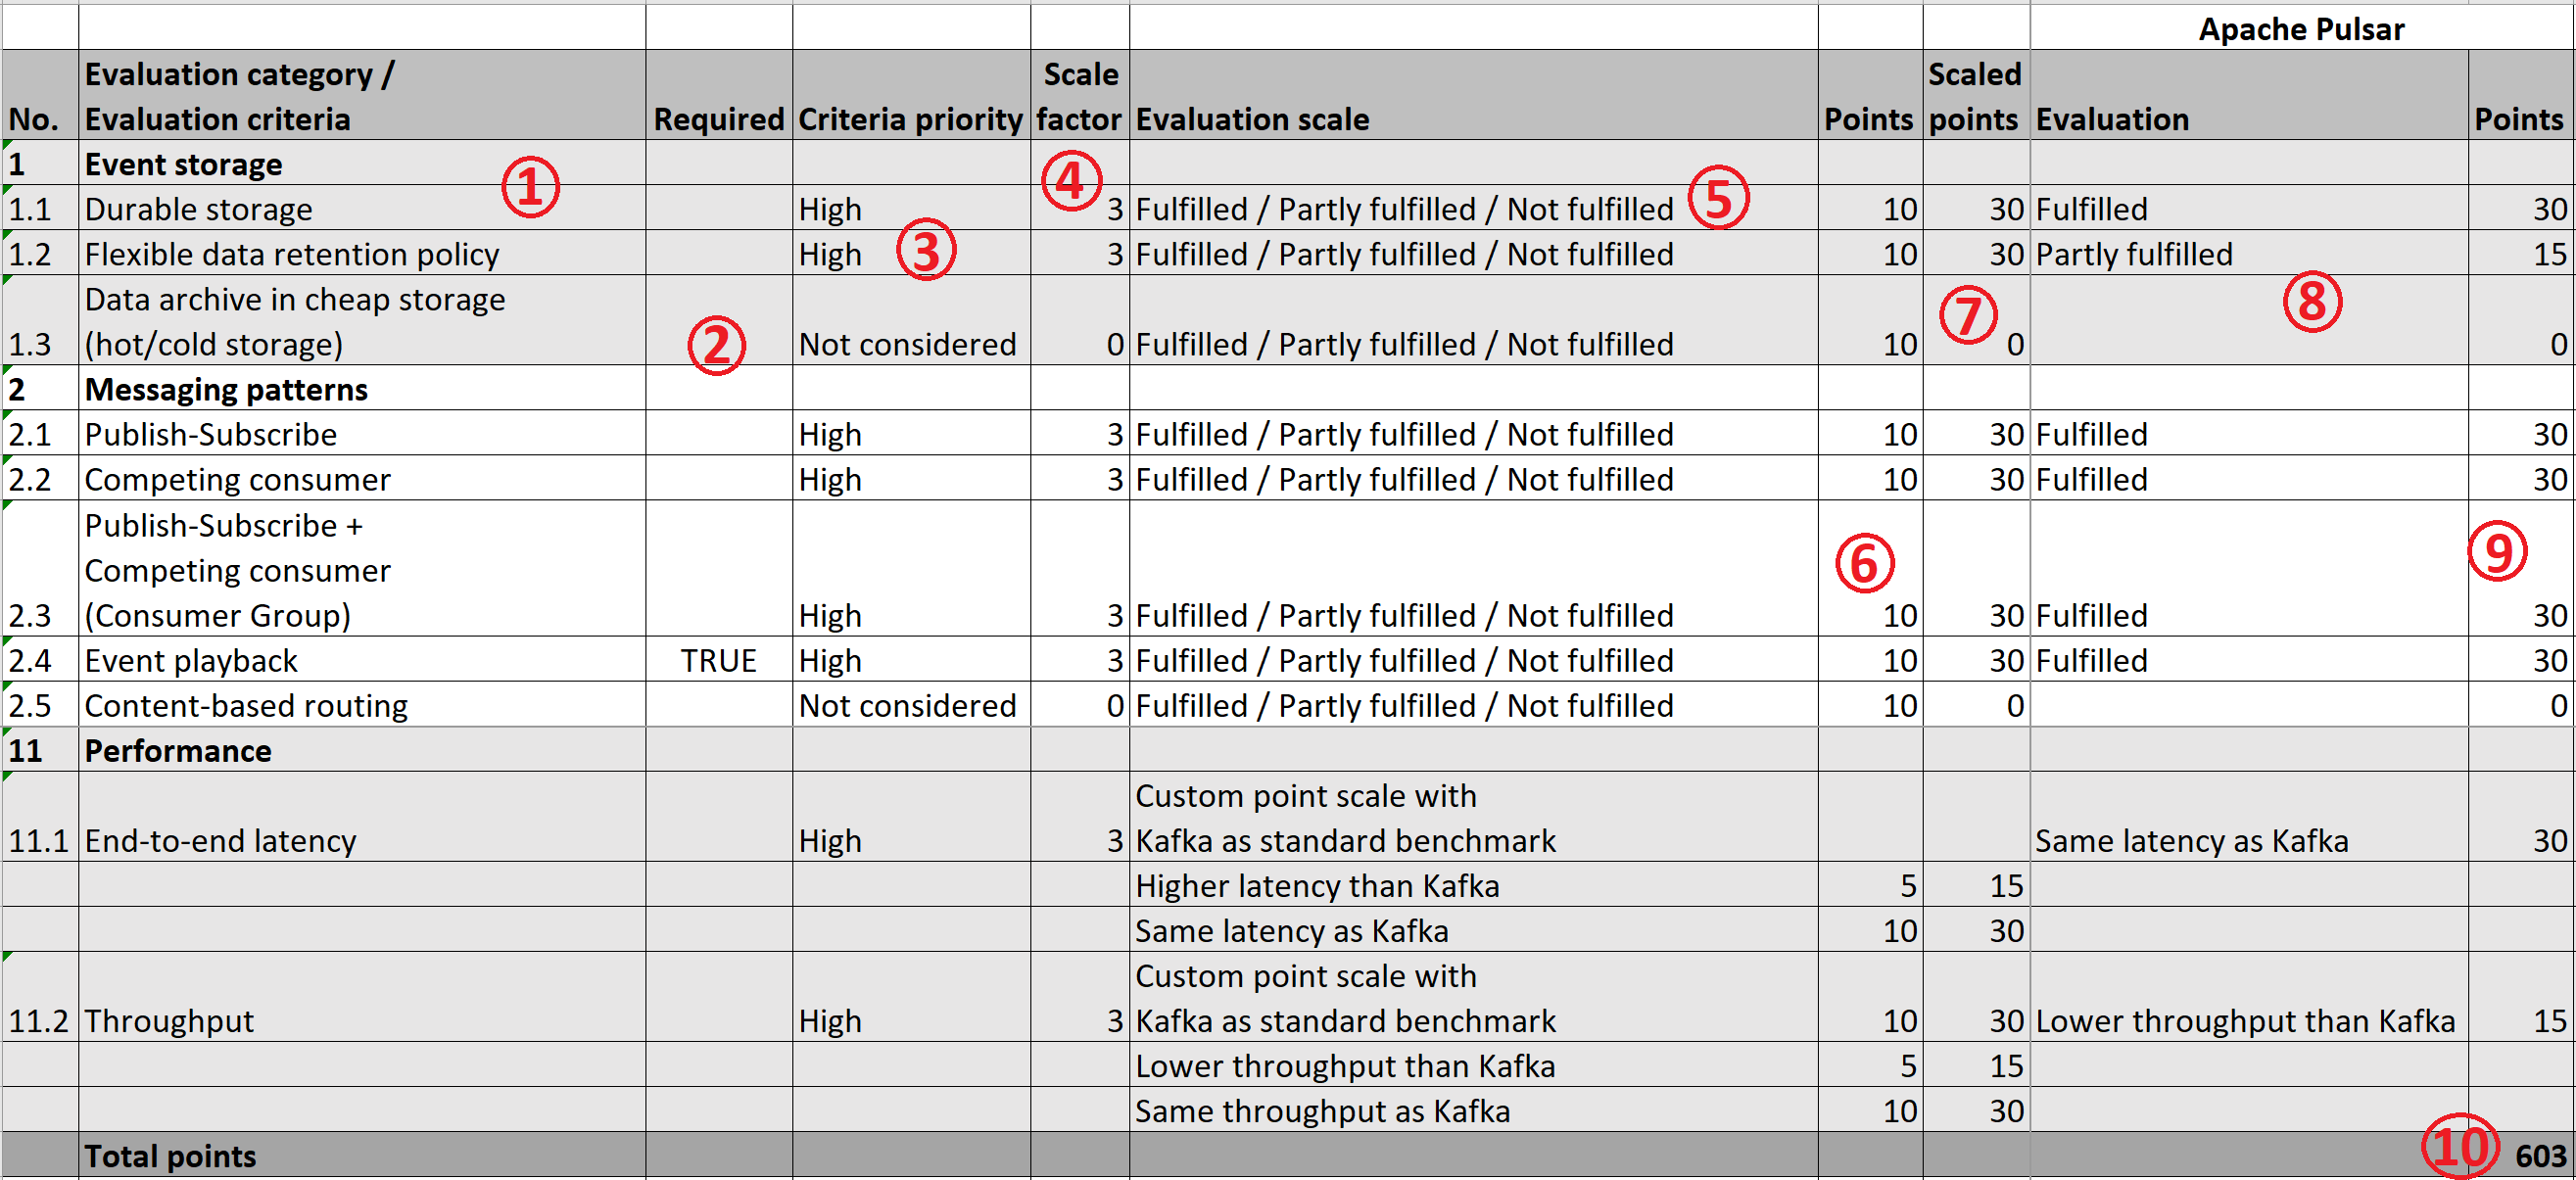
\includegraphics[width=18cm,height=8cm]{images/feature-matrix.png}
	\end{adjustwidth}
	\caption{General structure of the feature matrix.}
	\label{fig:featurematrix}
\end{figure}

The main components of the matrix are elaborated in the following:
\begin{itemize}
	\item 1: This column indicates the evaluation categories and the corresponding criteria of each of them.
	\item 2: In this column, users have the possibility to specify a specific criterion to be vital in their use cases. For instance, in figure \ref{fig:featurematrix}, the \emph{Event playback} criterion is set to be required. Any platform which does not fulfill this criterion will be immediately eliminated from the evaluation results.
	\item 3: The priority of each evaluation criterion can be defined on this column. There are 4 different levels of priority: \emph{High / Medium / Low / Not considered}. In the matrix, all evaluation criteria defined in section \ref{section:evaluationcriteria} are included and the metrics which are not evaluated in the thesis are marked as \emph{Not considered}.
	\item 4: Based on the priority level in column 3, each evaluation criterion is assigned a weighting factor as follows: \emph{High} - 3, \emph{Medium} - 2, \emph{Low} - 1, \emph{Not considered} - 0. The criteria which are not considered are essentially granted the points of 0 to have no effect on the final evaluation point.
	\item 5: This is where the evaluation scale of each criterion is defined. There are two types of evaluation scale. The first is standard scale: \emph{Fulfilled / Partly fulfilled / Not fulfilled}. The second is custom scale which is only applicable to a specific criterion (e.g. the custom point scale of the \emph{End-to-end latency} criterion in figure \ref{fig:featurematrix}). 
	\item 6: In this column, the unweighted points without considering the priorities of the criteria are defined in the range from 0 to 10 according to the evaluation scale on column 5. With the standard scale, the mapping from evaluation scales to unweighted points is as follows: \emph{Fulfilled} - 10, \emph{Partly fulfilled} - 5, \emph{Not fulfilled} - 0. For custom scale, the mapping is defined explicitly in the matrix. 
	\item 7: In this column are the weighted points of the criteria by multiplying the scaling factor in column 4 and the unweighted points in column 6.
	\item 8: In this column are the actual evaluation results of the platforms according to the defined evaluation scale.
	\item 9: This is the weighted point granted to the platform for each of the evaluation criterion.
	\item 10: For each platform, the weighted points of all considered evaluation criteria are summed up and presented as the final evaluation point.  
\end{itemize}

With this structure of the matrix, users have the flexibility to adjust priorities of each criteria on column 3 and define which criterion is vital on column 2. The returned total points can help decide which platform is most suitable for the requirements of users.